%% Dokumentenklasse (Koma Script) -----------------------------------------
\documentclass[%
   11pt,              % Schriftgroesse
   english,           % wird an andere Pakete weitergereicht
   a4paper,           % Seitengroesse
   DIV12,             % Textbereichsgroesse (siehe Koma Skript Dokumentation !)
	 parskip=half
]{scrartcl}%     Klassen: scrartcl, scrreprt, scrbook
% -------------------------------------------------------------------------

\usepackage[latin1]{inputenc} % Font Encoding, benoetigt fuer Umlaute
\usepackage[english]{babel}   % Spracheinstellung

\usepackage[T1]{fontenc} % T1 Schrift Encoding
\usepackage{textcomp}    % Zusatzliche Symbole (Text Companion font extension)
\usepackage{lmodern}     % Latin Modern Schrift

%% [OPT] Easily changeable quotes with \enquote{Text}
\usepackage[babel]{csquotes}

%% [NEED] This allows for additional typesetting tools in mathmode.
%% See its excellent documentation.
\usepackage{mathtools}
\usepackage{mathbbol}


%\usepackage{subcaption}


%% [REC] Nicer tables.  Read the excellent documentation.
\usepackage{booktabs}

%% [CUSTOM LW] Text Color
\usepackage{color}
\usepackage[usenames,dvipsnames]{xcolor}

%% [CUSTOM LW] Typesets chemical formulae
\usepackage[ghsystem=false]{chemmacros}

%% [CUSTOM LW] Enable custom lists
\usepackage{xstring}

\usepackage[inline]{enumitem}

%% [CUSTOM LW] BibLaTeX
\usepackage[sorting=none,backend=biber,maxcitenames=1,maxnames=1,firstinits,url=false,isbn=false,eprint=false,doi=false]{biblatex}
\bibliography{refs}

%% [CUSTOM LW] IEEEeqnarray
\usepackage[retainorgcmds]{IEEEtrantools}

%% [CUSTOM LW] Subfloats
\usepackage{subfig} % for subfigures
\usepackage{caption}

%% [CUSTOM LW] Bold Math
\usepackage{bm}

%% [CUSTOM LW] Long Tables
\usepackage{booktabs}
\usepackage{longtable}
\usepackage{tabu}

%% [REC] Fancy character protrusion.  Must be loaded after all fonts.
\usepackage{microtype}

\usepackage{import}

\usepackage[hidelinks]{hyperref}

\pdfstringdefDisableCommands{%
  \renewcommand{\color}[2]{#2} % this causes the warning for \kern
}

%% [CUSTOM LW] Maximum Page Numbers for Research Plan
\newif\ifMaxPages
\MaxPagesfalse
%% \MaxPagestrue
\newcommand{\onlyIfMaxPages}[1]{\ifMaxPages{\color{red}{#1}}\fi}

%% Section Spacing
%% \RedeclareSectionCommand[beforeskip=-2.5ex plus -1ex minus -.2ex, afterskip=.1\baselineskip]{section}
%% \RedeclareSectionCommand[beforeskip=-1.5ex plus -1ex minus -.2ex, afterskip=.1\baselineskip]{subsection}
\RedeclareSectionCommand[beforeskip=-1.0ex plus -1ex minus -.2ex, afterskip=.0001\baselineskip]{subsubsection}
%% \RedeclareSectionCommand[beforeskip=.001\baselineskip, afterskip=-1em]{paragraph}

%% Subfigure Layout
% \captionsetup{labelfont={bf, footnotesize}, textfont=footnotesize}
\captionsetup[subfigure]{labelfont={large,bf,sf},singlelinecheck=off,justification=raggedright, labelformat=simple, position=top}
\renewcommand{\thesubfigure}{\Alph{subfigure}}
\usepackage{macros}

%% Dokument Beginn %%%%%%%%%%%%%%%%%%%%%%%%%%%%%%%%%%%%%%%%%%%%%%%%%%%%%%%%
\begin{document}

\begin{titlepage}

\newcommand{\HRule}{\rule{\linewidth}{0.5mm}} % Defines a new command for the horizontal lines, change thickness here

\center % Center everything on the page
 
%----------------------------------------------------------------------------------------
%	HEADING SECTIONS
%----------------------------------------------------------------------------------------
\textsc{\LARGE Ph.D. Research Plan}\\[1.5cm] 
%\textsc{\Large Major Heading}\\[0.5cm] % Major heading such as course name
%\textsc{\large Minor Heading}\\[0.5cm] % Minor heading such as course title

%----------------------------------------------------------------------------------------
%	TITLE SECTION
%----------------------------------------------------------------------------------------

\vspace{1.4cm}
%\HRule \\[0.4cm]
%{ \huge \bfseries Flux distributions in metabolic networks}\\[0.4cm]
\setlength{\baselineskip}{25pt}
{ \huge \bfseries Sketching and Streaming Algorithms for Bioinformatics applications}
 % Title of your document
%\HRule \\[1.5cm]
 
%----------------------------------------------------------------------------------------
%	AUTHOR SECTION
%----------------------------------------------------------------------------------------
\vspace{3cm}

\begin{minipage}{0.4\textwidth}
\begin{flushleft} \large
\emph{Ph.D. Candidate:}\\
Amir \textsc{Joudaki} % Your name
\end{flushleft}
\end{minipage}
~
\begin{minipage}{0.4\textwidth}
\begin{flushright} \large
\emph{Supervisor:} \\
Prof. Dr. Gunnar  \textsc{R\"{a}tsch} % Supervisor's Name
\end{flushright}
\end{minipage}\\[4cm]

% If you don't want a supervisor, uncomment the two lines below and remove the section above
%\Large \emph{Author:}\\
%John \textsc{Smith}\\[3cm] % Your name

%----------------------------------------------------------------------------------------
%	DATE SECTION
%----------------------------------------------------------------------------------------

\textsc{ETH Z\"{u}rich} \\
Department of Computer Science\\
Biomedical Informatics Group\\
% \emph{Accepted:} September 2016\\
\emph{Started:} October 2019\\
% \onlyIfMaxPages{\\Total max. 10 pages}
%{\large \today}\\[3cm] % Date, change the \today to a set date if you want to be precise

%----------------------------------------------------------------------------------------
%	LOGO SECTION
%----------------------------------------------------------------------------------------

%\includegraphics{Logo}\\[1cm] % Include a department/university logo - this will require the graphicx package
 
%----------------------------------------------------------------------------------------

\vfill % Fill the rest of the page with whitespace

\end{titlepage}


\section{Summary\onlyIfMaxPages{ (max. 1/2 page)}}
Over the past two decades, there has been an exponential increase in the capacity of next-generation sequencing technologies~\cite{stephens2015big}. The magnitude of these sequence datasets has created a demand for statistics and machine learning algorithms that are capable of analyzing sequences, from hundreds of millions up to billions of nucleotides in length. Therefore, designing scalable algorithms and data-structures for bioinformatics application is the main focus of this research plan. 

Sketching and streaming algorithms are branches in algorithm design and provide a well-suited framework for designing scalable bioinformatics methods. Informally, streaming is a paradigm in which the algorithm takes one pass over the samples, and sketching refers to summarizing the relevant information during the pass. Crucially, memory complexity must remain sub-linear in the input size, since the input cannot fit into memory in its entirety. This assumption is necessary for many real-world datasets, such as multiple sequences alignment. The sketching-based algorithms are easy to implement and provide certain guarantees. These guarantees are often proved under realistic assumptions about data that can be independently verified. While sketching and streaming ideas have been successfully employed in information retrieval and compressive sensing, they have not been fully embraced by the bioinformatics community. Therefore, we set out to design algorithms and data-structures within the sketching and streaming framework, tackling computationally expensive problems such as inexact read to reference alignment, whole-genome alignment, multiple-genome alignment, synteny alignment, and visualization of genomes.

\onlyIfMaxPages{\pagebreak}
\section{Introduction\onlyIfMaxPages{ (min. 1/2 page)}}

The main ideas sketching algorithms rely on,     developed in different domains, such as the study of randomized algorithms and probabilistic methods, similarity preserving embeddings, compressive sensing, and sensitive hashing. For instance in compressive sensing, the discovery that sparse signal recovery requires fewer samples than predicted by the Nyquist-Shannon sampling theorem has allowed faster MRI acquisition by requiring fewer samples. In a nutshell, given the prior knowledge about sparsity and with the right sensor design, the recovery can be relaxed and solved via $\ell^1$-minimization methods, such as iterative thresholding. Other notable examples are min-hash, initially developed for detection of duplicate documents, and Bloom filters, developed for memory-efficient set membership queries when some false positives are acceptable. Despite the original use cases, both methods have found application in bioinformatics for classifying sequences and analysis when exact similarity estimation is not feasible. 


The techniques introduced above, have been utilized to lower the complexity of many important algorithms and optimization procedures, such as low-dimensional random features, convex optimization, and symmetric tensor sketching.
One of the main advantages of these probabilistic algorithms is that the accuracy-complexity trade-off can be computed, allowing us to design algorithms that are more predictable, interpretable, robust, and have fewer unknown quantities than more sophisticated models such as random forests and deep neural networks. 
Therefore, revisiting these mathematically rigorous but computationally inexpensive models can potentially lead to faster and more robust algorithms for bioinformatics applications with terabytes of data.



Due to the sheer scale and heterogeneous sources of variation in a genome, the exact alignment, or similarity estimation of sequencing reads is computationally intractable. Therefore, most tools rely on prior knowledge about the data and use heuristics tailored to the specific requirements of each application. 
However, relying on heuristics makes it harder to interpret the results, since it is not possible to know how sub-optimal the results are. 
In multiple sequence alignment, there is a complete lack of a gold-standard method with a run-time not growing exponentially with respect to the number of sequences. On the other hand, the assumptions for optimality of sketching-based algorithms are often explicit, and the sub-optimality ratio can be traded for time and memory complexity. 



The connecting theme of research goals outlined in this text is sketching distance metrics into $\ell^1$ or Hamming cube. These sketches will automatically lead to efficient nearest neighbor algorithms. Moreover, operating on vectors or bit-strings, can be optimized at the CPU or GPU level. The research goals and working packages follow a natural progression, since the main ideas in each section are developed on top of the previous ones. 


The first working package concerns sketching the similarity of strings. The edit operations, as defined by the edit distance, are a good proxy to evolutionary distances, caused by mutations. As an application, these sketches can be used to cluster short sequences belonging to multiple species, and to estimate distance between these genomes. The second step is to use the sketches and nearest neighbor queries, for read to reference alignment, using a seed and extend strategy. The sketches can be used to find the best seed, even if the seed contains a few point mutations. While the edit operations closely model genomic changes on the single nucleotides, the structural changes, such as translocation, inversion, or duplication, operate on a different scale. Therefore, in the third step we plan to build a syntenic sketch on top of similarity sketches, that captures such changes to the genome. The sketches can be used to find syntenic blocks and regions, as well as find syntenic alignments using nearest neighbor queries. Finally, one may generalize the two-level sketching for syntenic regions, to a multi-level recursive sketch. These sketches, combined with de-Brujin graph representation of sequences, may shed new light on genomic structural differences, as well as to visualize them. 



\onlyIfMaxPages{\pagebreak}
\section{State of the Art\onlyIfMaxPages{ (min. 1 page)}}

The most popular distance metric used in computer science and computational biology is Levenstein's distance, also referred to as \emph{the edit distance}, denoted by $\ED$ in this text. \cite{Levenshtein1966BinaryReversals}. Despite decades of research for faster exact algorithms, the quadratic time of the dynamic programming solution\cite{Vintsyuk1968SpeechProgramming}, has been only reduced to $\Ocal(n^2/\log^2 n)$, which essentially remains quadratic in the string length $n$ \cite{Masek1980ADistances}. This has spurred research on approximation algorithms, starting with a linear-time $\sqrt{n}$-approximation\footnote{An approximation factor $C$, implies computing an estimate metric $\D(x,y)$, that satisfies ${\ED(x,y)\le \D(x,y)\le C \cdot \ED(x,y)}$} by Meyers and Schmidt\cite{Landau1998IncrementalComparison}. Further research on quasi-linear\footnote{It means linear up to a polylogarithmic factor in input size $\Ocal(n\cdot \mathrm{Polylog}(n))$} algorithms has reduced this factor to $n^{3/7}$ by Bar-Yossef et al.~\cite{Bar-Yossef2004ApproximatingEfficiently}, to $n^{1/3+o(1)}$ by Batu et al.~\cite{batu2006oblivious}, and then vastly improved to $2^{\tilde\Ocal(\sqrt{n})}$ and ${(\log n)}^{\Ocal(1/\varepsilon)}$ by Andoni et al.~\cite{Andoni2012ApproximatingTime,Andoni2010PolylogarithmicComplexity}.  Finally, the only known strongly sub-quadratic result with an absolute constant approximation factor runs in $n^{2-2/7}$~\cite{Time2018ApproximatingTime}. 

Sketching the edit distance is a related and equally important problem. The goal is to  function that maps strings $x,y\in \abc^n$ to a binary string $\varphi: \abc^n\to \{0,1\}^m$, such that some distance between sketches, namely their hamming distance $\HD(\varphi(x),\varphi(y))$, approximates the edit distance $\ED(x,y)$, analogous to the approximation algorithms. For example an embedding into $\ell^1$ or Hamming cube, automatically leads to more efficient neighbor search algorithms, due to classical results by Indyk et al.~\cite{Indyk1998ApproximateNeighbors}. The best embedding result for the edit distance remains the $\ell^1$-embedding by Ostrovsky and Rabani with gives a $2^{\tilde\Ocal(\sqrt{n})}$-approximation . Eventhough this embedding has inspired some of the state-of-the-art results on approximating the edit distance, it is not known if the embedding itself can be computed efficiently. 


The edit distance and its variants, were first introduced to bioinformatics by Smith and Waterman~\cite{Smith1981IdentificationSubsequences}, since the edit operations can model \emph{single nucleotide polymorphism (SNP)}, \emph{indels (insertion or deletion)}, or sequencing errors in the DNA. However, due to the high cost of exact computation, several state-of-the-art tools rely on $k$-mers frequency~\cite{mapleson2016kat}, spaced $k$-mer frequency~\cite{morgenstern2019sequence}, and maximal matching substrings~\cite{thankachan2017greedy}, in order to estimate evolutionary distances. These distances and the position of substring matches can be used for phylogeny construction~\cite{thankachan2017greedy}, clustering multiple sequences~\cite{ondov2016mash}, read to reference mapping~\cite{chakraborty2019s}, and \emph{de novo assembly}~\cite{li2016minimap}. 


Evolutionary changes in the genome beyond SNPs and indels, such as inversion, duplication, and translocation, cannot be modeled correctly as edit operations, also referred to as \emph{structural variations}. Therefore, tools such as SyRI~\cite{goel2019syri}, find rearranged subsequences in assembled sequences, which might reside in a \emph{syntenic region}. Moreover, these structural differences are key to visualize assembled genome on different scales~\cite{Yokoyama2019MoMI}. 


Finally, sketching techniques have been successfully employed to lower the computational burden of many algorithms, such as fast \emph{Johnson-Lindenstrauss (JL)} dimensionality reduction~\cite{AILON2007THENEIGHBORS}, low-rank matrix factorization~\cite{tropp2017practical,yurtsever2017sketchy}, fitting kernel machines~\cite{rahimi2008random}, graph sparsification~\cite{spielman2011spectral}, and solving linear programs~\cite{cohen2019solving}, and efficient sketching of low rank tensors, can be exploited to fit polynomial kernels more efficiently~\cite{pham2013fast}. 


\subsection{Motivation}

% The increase in capacity of high-throughput next-generation sequencing technologies, has created a demand for efficient and scalable algorithms. 
The size of datasets produced by  high-throughput next-generation sequencing technologies, typically exceeds the available memory, which renders algorithms that require random access to the entire dataset inapplicable.
Therefore, in one or a few passes over the sequence, the most relevant information must be extracted and stored. 
This summary information must suffice to approximately answer queries relevant to the application.  
Sketching and streaming algorithms follow a similar paradigm, and often lead to practical and easy to implement algorithms. This motivates us take to a similar approach to design efficient algorithms for important problems in bioinformatics. 


\onlyIfMaxPages{\pagebreak}
\section{Goals of Thesis\onlyIfMaxPages{ (min. 1 page)}}\label{sec:goal_of_thesis}

This proposal aims at designing efficient algorithms for large-scale bioinformatics applications. The broad goals are:
\begin{itemize}
    \item  \textit{Sketching sequence similarity:} Sketching can be used to estimate similarity, and  for efficient clustering of sequences.
    \item \textit{Sketch-guided alignment:} Both read to reference alignment, and local alignment of multiple references can benefit from the pre-computed sketches.
    \item \textit{Syntenic region finding:} A hierarchical sketching method can capture similarity of sequences on a longer range.
    \item \textit{Multi-scale visualization: } The goal is visualization of sequence graphs constructed for multiple reference genomes, with multiple levels of abstraction.
    % \item \textit{Sketching-based optimization:} Exploring sketching ideas to make important optimization procedures more efficient. 
\end{itemize}


\subsection{Sketching sequence similarity}
The main focus in this part is the analysis of sequence data and using sketching methods for 
\emph{Sequence similarity sketching.} The distance between two genomes involves finding a alignment, that requires $\Ocal(mn)$ time complexity, in which $m$ and $n$ are genome lengths. However, it is possible to estimate the distance in a fraction of the time needed for the exact computation. The goal here is to design and test algorithms that estimate Levenshtein's distance, with quasi-linear time and memory complexity. 

 \emph{Classifying sequences:} The sketch values, both for edit distance and spaced $k$-mers, can be directly used to estimate distances between short sequences, reads, or $k$-mers, to estimate pairwise or group-wise genome distances, comparable to the Jaccard-based similarity estimation in MASH\cite{ondov2016mash}, yet more robust to mutations and sequencing errors. The results can be compared to other alignment-free distance estimation methods, mainly when genomes are not closely related. 

\textit{Spaced $k$-mers} enhance sensitivity of sequence analysis to high mutation rate by masking out a pre-defined subset of positions, sometimes referred to as \emph{don't care} positions. Although this is a more restrictive definition of string similarity, spaced $k$-mers are easier and more practical to implement. One limitation of spaced $k$-mers is that their sensitivity depends on the don't care pattern. This limitation motivates the following question: Is there an encoding which is as good as any $k$-mer pattern? This problem, can be studied as extension and specialization of the original sketch.  


\subsection{Sketch-guided alignment}
While sketching is not an alignment algorithm, it can be combined with alignment methods in order to lower their time complexity. The \emph{seed and extend} strategy for aligning a sequence read to a reference sequence, leads to an exponential growth in time complexity as a function of the number of mismatched characters. In some methods, bounded worst-case performance is achieved by having a bounded search time, at the expense of suboptimality of the alignment. 
Sketching of sequences into $\ell^1$ or Hamming cube $\{0,1\}^m$ can be used to speed up search for the best seed, using ideas from locality sensitive hashing. 
The sketch values can be precomputed and be reused for all subsequent computations. If sequences are stored as a de-Brujin graphs, these sketches can be stored as vertex colors, or in a separate hash table.  


 

\subsection{Syntenic region finding}
\emph{Syntenic regions} are coarsely related regions across two or multiple reference sequences, that contain multiple closely related \emph{syntenic blocks}. 
Syntenic regions may span few thousand to hundreds of thousands nucleotides. 
Identifying syntenic regions and blocks is essential for characterization of genomic differences in recently diverged species~\cite{vergara2010large}. 
Syntenic regions may contain genes are subject to inversions, duplication, or translocation, as well as long, unrelated sequences (gaps).
Due to these structural variations, finding syntenic regions and aligning syntenic blocks across multiple genomes is challenging.


The edit distance can be the similarity metric for syntenic blocks, and the the number of aligned blocks can be used to define syntenic region score. However, 
The main goal of this part, is to devise a hierarchical sketching scheme on top of the edit distance sketch, such that regions that share multiple similar blocks are given similar sketches. 
Such a sketch is ideally tolerant to some mismatches in syntenic blocks, and can be combined with sensitive hashing to identify  syntenic regions across multiple regions. 

  
de-Brujin graphs efficiently identify perfectly conserved recurring $k$-mers in our dataset. However, $k$-mers are too sensitive to mismatches, as well as genes subject to structral variations. Therefore, syntenic region sketches may reveal structural can be used to add extra ``similarity'' edges that indicate a coarse similarity between vertices, namely using a locality sensitive hashing scheme. Therefore, paths representing different genomes, will be joint at vertices designating a shared $k$-mer, and are ``bundled'' together by similarity edges, indicating syntenic region.


% Having addressed the computational challenges, help us understand evolutionary relationships that are difficult to capture with more traditional methods. Path bundles constructed on top of the de-Brujin graph can reveal complicated patterns of evolutionary history. As an example, horizontal gene transfer complicates any phylogeny based analysis. A gene may have several ancestors. Conceptualizing, computing, and visualizing these patterns can be an essential step in understanding the role of HGT in the evolution of viruses and bacteria, as well as antibiotic-resistant bacteria. 
% \end{itemize}

\subsection{Multi-scale, multiple genome visualization}

While visualization is not a scientific problem per se, it can help researchers to gain better insight into structural variations in whole genomes, across multiple species.
However, visualizing a de-Brujing graph across multiple ``scales'' requires an objective. Any definition of path-bundles or syntenic region, requires the acceptable level of similarity in a region. There will be a natural trade-off between the similarity parameter and the length of a block. Therefore, syntenic regions computed for different similarity values, can be used to visualize the genomes for different scales. 
An alternative more efficient strategy, is to compute a minimal set of spanning trees that preserve the structure or shortest distances in the graph.

% These trees may also offer an alternative to the phylogeny tree when a single tree is insufficient to capture intricate differences between subgroups. 
% This problem can be studied in conjunction with path bundles, as they offer an abstraction of de-Brujin graphs on differing levels, e.g., one possibility is to build the trees on top of path-bundles. One must tune the model hyper-parameters to get the desired abstraction. 
% However, both path bundles and tree spanners, are biologically motivated and not mathematically well defined.  Therefore, this step involves addressing modeling and computational challenges. 



% \textit{Graph-informed, sequence similarity estimation:}
% In many applications, one needs to quantify how dis/similar two species or groups of species based on their genome sequences. While the definition of dis/similarity varies from one application to another, traditionally, cheap to compute quantities are used as proxies for the real distance, such as approximate $k$-mer Jaccard distance. Given the non-trivial global and local patterns present in de-Brujin graphs, one can strive for better graph-inspired approaches to similarity. There is a vast literature on properties of biological networks as a starting point, while statistical and machine learning models can be employed to link graph properties. For example, to study if certain network motifs that are only present in a subgroup of specifies, one may use a dictionary of motif counts in graphs to predict the subgroup or subspecies types. The computational complexity remains an important issue, as many quantities are expensive to compute naively. 

% \end{itemize}



% \subsection{Sketch-based optimization}
% Sketching and compressive sensing inspired techniques have been successful in lowering the complexity of many important optimization algorithms. That said, there are still many resolved problems and unexplored direction, which is broadly the goal of this section. 

% \begin{itemize}
%     \item Recent developments show how to sketch rank one efficiently, or super-symmetric tensors, i.e., the permutation of indices will not change the value. These sketches have desirable properties, such as tensor contractions become vector products, and are optimally oblivious norm preserving, making it possible to operate in the low-dimensional space entirely. Furthermore, random-projections translate to FFT and inverse FFT operations, significantly reducing the time complexity. The key ingredient, however, is that these quantities can be computed recursively, which may substantially expand the class of tensors that admit efficient sketching. Given that tensors are versatile objects that are present in many optimization algorithms and machine learning models, any algorithmic improvements for implicitly operating with tensors can trickle down to various applications. 


%     \item Kernel methods and random Fourier features as their low dimensional counterparts have been influential in continuous optimization techniques in the past. Technical differences aside, the promise of looking at the problem in the high dimension is that it becomes more tractable/separable/decomposable. We propose to pursue this approach for combinatorial problems, while an analog to random Fourier features will avoid the full cost of solving the high-dimensional problem. The tensor sketching method developed in the previous step is the first step towards efficient approximation algorithms for \begin{enumerate*} \item counting common subsequences of a certain length \item count induced cliques of a constant size \end{enumerate*}
%     While these algorithms may not beat the state-of-the-art methods, they have the advantage of being more generic and are much more versatile. For example, modifying the algorithm to have gap and mismatch penalties will be trivial in this setting, while in general, this is a non-trivial problem. 
    
    
%     \item While compressive sensing inspired methods are successfully applied to lower the complexity of optimization algorithms, less research has focused on their statistical properties.  For example, lowering the input dimensionality in effect shrinks the number of parameters. While technically simple, this may give a fundamentally different insight about randomized dimensionality reduction, in that they simultaneously lower the complexity and regularize the model. One may strive to implement various regularization types, by random projections or sub-sampling methods. 
    
%     \item Multivariate polynomials are able to approximate complicated functions with only a few parameters. Equipped with ordinary differential equations, they are known to describe the behavior of many dynamical systems. Sparsity constraints successfully prevent overfitting~\cite{brunton2016discovering}. The problem, however, is that the complexity of all these methods grows exponentially with the degree of the polynomial, rendering it inapplicable for datasets with thousands of variable and real-time applications that expecting the results in a matter of seconds. Sparse polynomial regression, relaxed to $\ell^1$, can be computed in time polynomial as a function of the maximum degree.
    
    
%     \item As an extension to the previous step, one does need to restrict the class to polynomials. In a similar spirit to dictionary learning, one can introduce more types of features, but enforce sparsity to avoid over-fitting, say with $\ell^1$ relaxation. The in-sample error rate of this model grows logarithmically with the number of features, and the exponential requires a polynomial number of samples to fit. As a potential application, the governing equations of many dynamical systems are known to have only a few terms, and with sufficient data, the parameter and structure search is feasible. We aim to drive down the time complexity while keeping the advantages. 
    
%     \item Both methods above can be alternatively seen as a neural network. For example, polynomial regression relates closely to sum-product networks, albeit with a different learning scheme. Therefore, if the sketching-based learning algorithm proposed, does so with theoretical guarantees, it would be a step towards building robust neural network models, and shed light on the conditions under which the model works. 
    
    
%     \item Network abstractions are ubiquitous in computational biology, protein-protein interaction, gene co-expression, and gene regulatory networks. More broadly, networks are powerful tools to explain the interaction between observed and unobserved variables. The main challenge, however, is that we do not know the structure of the network in advance, simultaneously presenting a modeling and computational problem. The modeling problem is due to noise and scarcity of data, which, combined with exponential search space for structure, leads to overfitting. This problem is more pronounced when considering interactions between more than two variables and allowing different types of interaction. In structural inference modeling involving fitting differential equation parameters, a similar approach to sparse polynomial regression can be adopted to lower the complexity. 
    
%       \item \textit{Motif finding in networks:} Although conceptually different, from a combinatorial perspective, network motifs are graph counterparts to \emph{common subsequence} on strings. Therefore, the tools developed for the former can be applied to compute or estimate network motifs of an arbitrary pattern. The goal is to answer queries of type: how many cliques of size five $K_5$, does it contain as induced sub-graphs? Queries can be paired with metadata, such as vertex or edge colors. Given the streaming paradigm, the algorithm must have strictly sub-linear memory complexity, and it is given a single pass over edge insertion and deletions. The approximation is acceptable in many scenarios, as the real data contains inherent noise and other types of noise. 

    
    
% \end{itemize}

\onlyIfMaxPages{\pagebreak}
\section{Detailed Work Plan\onlyIfMaxPages{ (min. 1/2 page)}}


\subsection{WP1: sequence similarity sketching}
In this working package, the main objective is to sketch string similarity and output a concise binary string, such that the hamming-distance would gracefully increase as the strings become more dissimilar. Let metric $\D \colon \abcstr\times \abcstr\to R^{\ge 0}$ denote a string metric of interest, namely the edit distance. We look for a sketching function $\Sk\colon \abcstr\to\Set{0,1}^m$, such that for arbitrary strings $x,y\in \abcstr$, $\D(x,y)\approx \HD(\Sk(x),\Sk(y))$, in which $\HD$ stands for the \emph{Hamming distance} $\HD(x,y):=\#\{i\colon x_i\neq y_i\}$. One way to quantify the approximation is via \emph{distortion factor $\alpha>0$}, which informally means that the sketch-based estimate of distance is within a multiplicative $\alpha$-factor of the true distance. 
Formally, $\varphi$ has distortion $\alpha$, if there exists absolute constant $c$, such that for arbitrary strings $x,y\in S$, and distance threshold $t\in\RR^{\ge 0}$, there exists $t'\in\RR^{\ge 0}$ such that: 
\begin{equation}
\label{eq:sk_approx_factor}
\begin{cases} 
\Prob{\HD(\varphi(x),\varphi(y))> t'}\ge 1-\E^{-c \; m},& \text{if }  \D(x,y)>\alpha t\\
\Prob{\HD(\varphi(x),\varphi(y))\le t'}\ge 1-\E^{c \; m}, & \text{if } \D(x,y)\le t.
\end{cases}
\end{equation}
We can interpret \eqref{eq:sk_approx_factor} as the distortion $\alpha$ determines how much the distances can be expanded spuriously due to the sketching. 
Although the definition given here treats distortion as a constant, it is not always achievable, and $\alpha$ may depend on distance threshold $t$, sequence length $|x|,|y|$, or other parameters: $\alpha(t,|x|,|y|)$. \emph{Optimal sketching} implies that $\Sk$ achieves $\alpha=\Ocal(1)$-distortion using constant sized sketch $m=\Ocal(1)$.  


\subsubsection*{Sequence clustering}
One application for string sketching, is to cluster a large number of sequences, namely raw sequence reads, or metagenomic sequences. 
Let $S:=\Set{(s_i,g_i)}_{i\le N}$ be the list of $N$ sequences $s_i\in \abcstr$, along with their respective taxonomy code $g_i\in G$, and $S_g$ denotes the sequences belonging to $g$ $S_g:=\Set{s_i\colon g_i=g}$ The task is to estimate pairwise similarities between groups. Let us assume we interested in inter-group similarity $\Jacc_t(g,g')$ defined as number of sequences between groups $g,g'\in G$ that are $t$-close:
\[
\Jacc_t(g,g'):= \#\Set{(s_i,s_j)\in S_g\times S_{g'}\colon \D(s_i,s_j)\le t},  \qquad \norm{\Jacc_t}_1=\sum_{\Set{g,g'}\subseteq G} \Jacc_t(g,g')
\]
Definition for $J_t$ can be interpreted as soft-Jaccard similarity, as it allows for distance up to $t$ to be incorporated in similarity. If $\D(x,y)$ is the edit distance, the naive approach requires $\binom{N}{2}$ calls to the distance function $\D(x,y)$, which is prohibitive in both $N$ and length of the sequences $|x|,|y|$. Our goal to make the number of distance calls dependent on number of $t$-similar sequences, which can be substantially smaller $\norm{\Jacc_t}_1\ll N^2$. Instead, we pre-compute sketches $H:=\Set{(s_i,g_i,h_i), h_i=\Sk(s_i)}$. Due to the decay rate $\E^{-c m}$ in \eqref{eq:sk_approx_factor}, using $m:=\Ocal(\log(N))$ sized sketch suffices to have the property for for all pairs $s_i,s_j\in S$ simultaneously. Therefore, single-bit match probability $p_1$, for $t$-similar pairs, versus match probability $p_2$, for $\alpha t$-dissimilar string pairs:
\begin{equation}
\label{eq:bit_match_prob}
p_1=\min_{i\neq j}\Set{1-\frac{1}{m}\HD(h_i,h_j)\colon  \D(s_i,s_j)\le t},
p_2=\max_{i\neq j}\Set {1-\frac{1}{m}\HD(h_i,h_j) \colon \D(s_i,s_j)\ge \alpha t},
\end{equation}
A consequence of having \eqref{eq:sk_approx_factor} for all pairs is that $p_1>p_2$ with high probability. 
Using random bit-sampling, we can amplify the ratio $\frac{p_1}{p_2}$. We construct $L$ blocks, $I_1,\dots,I_L$, each of size $\ell$. To construct $I_j=\{i_1,\dots, i_\ell\}$ select each bit \iid and \uar from the set of all bits: $i_1,\dots,i_\ell\sim\Unif[m]$. Let $h_{i|I_j}$ denote the $I_j$-induced sub-sketch $h_{i|I_j}:=h_i[i_1] h_i[i_2] \dots h_i[i_\ell]$. Using the bit-collision probabilities \eqref{eq:bit_match_prob}, we can calculate the block collision probabilities.  
For all $k\in[L],i,j\in[N]$, we have:
\begin{align*}
&\Prob{h_{i|I_k}= h_{j|I_k}}\ge 1-(1-p_1^\ell)^L=:P_1 &&\D(s_i,s_j)\le t  \\
&\Prob{h_{i|I_k}= h_{j|I_k}}\le 1-(1-p_2^\ell)^L=:P_2 &&\D(s_i,s_j)\ge \alpha t 
\end{align*}
With some calculation, it can be shown that for $L=c N^\rho, \ell=\log(N)$, in which $\rho:=\frac{\log(1/p_1)}{\log(1/p_2)}<1$, we achieve $(1-P_1)\lesssim \E^{-c}$, and $P_2\lesssim 1/N^2$ (for more details see~\cite{datar2004locality}).
Based on these observations, let collision set $H(g,g')$ be defined as:
\[
H(g,g'):=\Set{(s_i,s_j)\in S_g\times S_{g'}\colon \exists k\; h_{i|I_k}= h_{j|I_k}},
\]
which we can sweep over, and decide which pairs are $t$-close 
\[
\tilde\Jacc_t(g,g'):=\# \Set{(s,s')\in H(g,g')\colon \D(s,s')\le t }.
\]
Ten, with high probability
\[
(1-\E^{-c}) \Jacc_t (g,g') \le \tilde\Jacc_t(g,g') \le \Jacc_t (g,g'), \qquad \forall g,g'\in G,
\]
requiring at most $\norm{\Jacc_{\alpha t}}_1$ distance calculations, can be substantially smaller than pairwise distance calls $\norm{\Jacc_{\alpha t}}_1\ll N^2$. 



\paragraph{Deliverables}
\begin{itemize}
\item A publication describing the method for string edit distance sketching, as well as specialized cases for gapped Hamming and shifted Hamming distance. 
\item An efficient implementation of the sketching method, plus experiments on some real-world genome datasets.
\end{itemize}

\newcommand{\AlgG}{\mathcal{A}_G}
\newcommand{\AlgL}{\mathcal{A}_L}
\newcommand{\AlgLG}{\mathcal{A}_{LG}}
\newcommand{\AlgGL}{\mathcal{A}_{GL}}

\subsection{WP 2: Sketch-based alignment}
The sketching framework which we developed on in the last working package, can be used to guide read to sequence alignment. Let us introduce some notation in order to define an alignment. Let $X,Y\subseteq \NN^{+}$ denote index sets, and $X_0:=X\cup\Set{0}, Y_0:=Y\cup\Set{0}$ append them with $0$. The precedence relation $\prec$ is defined as 
\[
(x_0,y_0)\prec(x_1,y_1) \iff ( x_0<x_1\wedge y_0<y_1) \vee (x_0<x_1 \wedge y_1=0) \vee (y_0<y_1 \wedge x_2=0)
\]
Alignment family $\Align(X,Y)$ is defined as set of all binary relations $\pi\subseteq X_0\times Y_0$, such that $\prec$ imposes a strict total order over $\pi$, and domain and co-domain of $\pi$ contain $X$ and $Y$ respectively. Alignment executions $\pi_1,\pi_2$ are defined as $\pi_1:=i_1,i_2,\dots,i_{\pi}$ and $\pi_2:=j_1,j_2,\dots,j_{|\pi|}$, where $(i_1,j_1)\prec (i_2,j_2)\prec \dots \prec (i_{|\pi|},j_{|\pi|})$ are members of $\pi$. 

For arbitrary strings $s,r\in\abcstr$, and $\pi\in\Align([|s|],[|r|])=:\Acal(s,r)$ define sequence executions as $s_{|\pi_1}:=(s[i_k])_{i_k\in \pi_1}$ and $r_{|\pi_2}:=(r[j_k])_{j_k\in \pi_2}$, where it is assumed $r[0],s[0]:=\veps$. Finally, we can define the optimal alignment:
\begin{equation}
\label{eq:optimal_alignment}
    \pi^\star(s,r) = \argmax_{\pi\in\Align(s,r)} f(s_{|\pi_1},r_{|\pi_2}).
\end{equation}
The alignment score $f(s_{|\pi_1},r_{|\pi_2})$, typically can be written as a function of the mismatch matrix $f(s_{|\pi_1},r_{|\pi_2})=\sum_{k=1}^{|\pi|} m(s[i_k],r[j_k])$, where $m:\abc_\veps^2\to\RR$ determines the penalty for gaps and mismatches. 

\subsubsection*{Guiding alignment}
It is straightforward to see that the optimal global alignment \eqref{eq:optimal_alignment}, corresponds to the edit distance if we set the $m(a,b)\gets -\1[a\neq b]$, which has a dynamic programming solution running in $\Ocal(|s||r|)$. This is considered inefficient if the query $s$ is significantly shorter than the reference $r$. If we can find the optimal starting position on the reference sequence, the complexity will be lowered to $\Ocal(|s|^2)$, since the distance cannot exceed $|s|$. 

Many alignment procedures, break the query and reference into $k$-mers as pre-processing steps in order to estimate the . For $d$-mismatches, at most $d(k-1)$ $k$-mers are touched by mismatching characters, and $|q|-(d+1)(k-1)$ are unaffected. These $k$-mers can act as anchors, where we base our alignment algorithm on. The advantage of these methods is $k$-mer exact matching can be implemented efficiently using a hash-map. The challenge is that if $k$ is too small, there will be instances of each $k$-mer, and it is not trivial how to choose the anchor, while a big $k$ risks having no untouched $k$-mer $|q|-(d+1)(k-1)\le 0$.

We propose sketch-match as opposed to $k$-mer match to be used as anchors. Let $\Set{(s_i)}_{i\le N}$ and $\Set{(r_i)}_{i\le M}$ denote $k$-mers of $s$ and $r$ respectively. Define the pair $(s_i,r_j)$ is an anchor if  $d(s_i,r_j)\le t$, which relaxes the definition to have $t$ mismatches. Therefore, we can use the same techniques outlined in the previous working package, in order to achieve sub-linear search time. 


% In this case, the time complexity grows exponentially with respect to the number of mismatches. Roughly speaking, if alignment is computed for a query sequence up to a certain point, if the next characters cannot be matched, the naive solution requires checking every possible character for alignment. In worst case, this may lead to exhausting the entire reference dataset. Therefore, many heuristics have been introduced to avoid trying visiting all search paths, similar to $A^\star$ algorithm. 

% While we described alignment and sketching over sequences, the framework can be transferred to de-Brujin graphs. 
% More specifically, suppose the reference sequence is stored on a de-Brujin Graph, and we only have the naive alignment algorithm that tries all possible paths and assigns a score to them. Moreover, the sketch values are computed in such a way that if $\D(s_q,s_i)>t$ we are guaranteed to have $\HD(h_q,h_i)>t'$. Furthermore, the sketches are stored on a subset of the vertices, with another data-structure points to next available sketch. Finally, when there are multiple outgoing edges, we can use the pointers to find the next sketch and avoid paths that point to a sketch with hamming distance above $t'$.


% For the first objective, the method is implemented and evaluated using artificially generated datasets, that mimic real genome mutations. Next, we can use a naive aligner in order to find the path with the highest alignment score. The simple aligner merely appends matching characters, and searches the space in a depth-first fashion and when there is a mismatch. The method is evaluated by replacing the query search by other sketching methods and comparing the alignment score. 
% For the second objective, we choose an aligner that relies on a heuristic to prune wrong search paths. Therefore, sketches and their distances provide the guarantee for pruning. Finally, read to reference aligner, such as MUMmer~\cite{Marcais2018MUMmer4}, may be used as baselines.



\paragraph{Deliverables}
\begin{itemize}
\item An implementation, as well as a publication, for read to reference alignment, using sensitive hashing values.
\end{itemize}


\subsection{WP 3: Syntenic region finding}
Syntenic regions are long ranges in assembled sequences, that contain multiple closely related syntenic blocks. Moreover, these blocks may be inverted, translocated, or duplicated, due to evolutionary recombination or other factors. The concrete goal of this working package to devise a locality sensitive hashing scheme, to find and align these syntenic regions. However, before we can design such a scheme, we need to formally define a syntenic region. 

Let $K$ denote the length of syntenic region, $k$ denote the syntenic block length, and $\rho_t(x,y)$ denote the similarity between $x$ and $y$ based on their edit distance, with $t$ as similarity threshold, and $\rho_t(x,y):=\1\{\ED(x,y)\le t\}$ be the hard-thresholding operator, indicating if $x,y$ are $t$-close ($1$) or not ($0$), and let $s[i:k]:=s[i,i+1,\dots,i+k-1]$ denote the $k$-mer starting at index $i$. Moreover, let $a, b\in \abc^K$ denote two syntenic regions, and $J$ designates the set of all monotonic pairings of $k$-mers:
\begin{equation}
\label{eq:def_monton_pairs}
\Align:= \Set{J\subseteq {\Ical\times \Ical}\colon \text{ if }  (i,j), (i',j')\in J,i\le i'\text{ then } j<j' }, \Ical:=\Set{1,1+k,1+2k,\dots}.
\end{equation}
The region score is formally defined as the maximum matching score between $a$ and $b$:
\begin{equation}
\label{eq:syntenic_region_score_sorted}
R(a, b,t) =  \max_{J\in \Align}
\sum_{(i,j)\in J}\rho_t(a[i:k], b[j:k]).
\end{equation}

\subsubsection*{Sketching the region score}
The region score \eqref{eq:syntenic_region_score_sorted} resembles the score function in Smith-Waterman algorithm. Let $\Sk:\abc^k\to \{0,1\}^m$ denote a sketch which for optimality ratio $c>1$, similarity threshold $t$, and collision probabilities $0\le q_2<q_1\le 1$, it satisfies:
\begin{equation}
\label{eq:ED_HD_LSH}
\begin{cases}
\ED(x,y)\le t\Rightarrow \frac{\HD(h_x,h_y)}{m}\le  1-q_1\\
\ED(x,y)\ge c t \Rightarrow \frac{\HD(h_x,h_y)}{m}\ge 1- q_2.
\end{cases}, 
\quad   x,y\in \abc^k, h_{\cdot}=\Sk(\cdot)
\end{equation}
Ideally, $q_2$ is as close to $0$ as possible, while $q_1$ is a constant larger than zero, namely $q_1>1/3$. Factor $c$ is the gap between upper and lower thresholds, which is preferably a constant close to $1$, and determines how sharp the detection is.  
Let $x_i,y_j$ denote $k$-mers $x_i=a[i:k], y_j=b[j:k]$ with sketches $h_i,g_j$ respectively, on which we define sequences
$H := h_1,h_{1+k},\dots,h_{K-k+1}$, and $G := g_{1},g_{1+k},\dots,g_{K-k+1}$.
We draw $\ell$ elements from $[m]$ uniformly at random with replacement, and repeat this process $L$ times, to construct bit-index sets $I_1,\dots,I_L$. These bit-index sets, induce sub-sketch strings $H[I_j]:=h_1[I_j],\dots,h_{K-k+1}[I_j]$, and $G[I_j]:=g_1[I_j],\dots,g_{K-k+1}[I_j]$, defined for all index sets $I_1,\dots,I_L$. 
The key idea is that the \emph{longest common subsequence (LCS)} of $H[I_j],G[I_j]\in \Set{0,1}^{\ell\star}$, is related to region score~\eqref{eq:syntenic_region_score_sorted}.

% Let $J^\star$ be the minimizer of $R(a,b,t)$, with cardinality $R=|J^\star|$, and for $i\in[R]$ define $S_i:=\Set{(x,y)\in J^\star \colon h_x[i]=g_y[i]}$. We have $\sum_{i=1}^m |S_i| \le R(1-q_1)m$. Let $|S_1|,\dots, |S_m|$ be in a non-decreasing order, $|S_i|> R(1-q_1) m/(m-i)$ leads to the contradiction $\sum_{j=i+1}^m |S_j| > R(1-q_1)m$. By union bound $\Abs{\cup_{j=1}^i S_j}\le  R(1-q_1)m i/(m-i)$, it is upper bounded by $\Abs{\cup_{j=1}^i S_j}\le R(1-q_1)m^\alpha$, if we set $i=m^\alpha,\alpha<1$. If we draw $\ell$ elements from $[m]$, with $(i/m)^\ell=m^{-1+\alpha}$ probability 

Let $\Ecal_{i,j}$ for $r\in[L]$ indicate the event $\{h_i[I_r]\neq g_j[I_r]\}$ ($1$: if it is true, $0$ otherwise), and $J^\star$ is the minimizer of $R(a,b,t)$. We have $\EE\sum_{(i,j)\in J^\star} \Ecal_{i,j} =  \Abs{J^\star}\Prob{\Ecal_{i,j}=1}$, which by property~\eqref{eq:ED_HD_LSH} is at most $R(a,b,t) {(1-q_1^\ell)}$. Therefore, by Markov's inequality we have $\Prob{\sum_{(i,j)\in J^\star} \Ecal_{i,j} \ge 4R(a,b,t) {(1-q_1^\ell)}} \le 1/4$. Let $\Ecal_{i,j}^c$ be the complement event $\Ecal_{i,j}^c:=1-\Ecal_{i,j}$, and $J^c$ be the set of $tc$-distant indices $J^c:=\Set{(i,j)\in \Ical: \ED(x_i,y_j)\ge tc}$. Using property~\eqref{eq:def_monton_pairs}, we have $\EE \sum_{(i,j)\in J^c} \Ecal_{i,j}^c \le (\frac{K}{k})^2 q_2^\ell$, and by Markov's inequality we have $\Prob{\sum_{(i,j)\in J^c} \Ecal_{i,j}^c \ge 4(\frac{K}{k})^2 q_2^\ell}\le 1/4$. Finally, combining the two by union bound, if we set $\ln(1/q_1)\lesssim\ell\lesssim \ln(1/q_2)$, and $L=\log(1/\delta)$, with failure probability $\delta$, for at least one $r\in[L]$ it holds:
\begin{equation}
    \label{eq:LCS_sandwitch}
 R(a,b,t)(1 - p_1) \le \LCS(H[I_r],G[I_r]) \le R(a,b,tc) + (\frac{K}{k})^2 p_2,
\end{equation}
in which $0<p_1,p_2<1$ are constants depending on the sketching function optimality ratio $c$, and probabilities $q_1,q_2$. Finally, since LCS similarity 2-approximates the edit distance, we can invoke the sketching function $\Sk$ on the sequences $H[I_1],\dots,H[I_L]$ and $G[I_1],\dots,G[I_L]$. Finally, if we compute componentwise Hamming distance, and report the median, the bound~\eqref{eq:LCS_sandwitch} will hold.


In the first step, we must transform the methods outlined in this package to more concrete ones, while ensuring that they approximate the corresponding biological concepts. In order to verify that the method works as expected, we must create a synthetic sequence dataset that closely follows the assumptions and definitions. Finally, the algorithm can be applied to a real dataset and compared against other syntenic aligners.  


\paragraph{Deliverables}
\begin{itemize}
\item An implementation of this approach, with application on simulated data, and two whole-genome references that are not very closely related. 
\end{itemize}


\subsection{WP 4: Multi-scale graph backbone and visualization}
% Given a de-Brujin graph $G=(V,E)$, informally, we want a ``simple`` sequence graph $T$, such that for sequences in $G$, there is a corresponding sequence in $T$ that approximates it. While the primary goal of constructing $T$ is visualization, it can also represent major variations in the set, or clean a graph constructed from raw reads. Hypothetically, a concatenation of all the reference sequences as a long simple chain contains all reference sequences with no error, yet offers no further insight about the sequences. This motivates us to put some constraint on the size of $T$. We proceed by proposing a possible formalization:


% \subsubsection*{Minimum dominating set}
% Formally, $G=(V,E)$ is the de-Brujin graph and $v\in V$ are $k$-mers, and $w(v)$ denoting the multiplicity of this $k$-mer in all our reference sequences, and for vertices $u,v\in V$, $\D(u,v)$ denotes the shortest path distance on the graph. Moreover, $\mathcal{N}(v,k)$ denotes its $k$-step neighborhood of a vertex $\mathcal{N}(v,k):=\{u\in V\colon \D(u,v)\le k\}$, which can be extended to a subset of vertices $\mathcal{N}(S,k):=\cup_{v\in S}\mathcal{N}(v,k)(v,k)$ for $S\subseteq V$. We call such a subset $(C,k)$-dominating if $\sum_{v\notin \mathcal{N}(S,k)} w(v)\le C$, and let $\mathcal{D}(C,k)$ denote all $(C,k)$-dominating sets with minimum cardinality ($|S|$ is the least possible). 
% If $S\in \mathcal{D}(C,k)$, the sequence graph induced by $v(S)$ has $|S|k$  characters,  and sum of the minimum distance of any $k$-mer in the reference sequences to $v(S)$ is bounded by $C$. 
% This optimization problem is NP-hard, as it contains a minimum dominating set problem as a special case. However, it admits approximation schemes that are efficient to compute. 

\subsubsection*{Sketch-based visualization}
The sketching scheme for syntenic region score can be readily used for visualization purposes. The first step is to visualize each genome sequence as separate paths, and if a syntenic region is found in multiple genomes, they will be joint at that location and diverge afterwards. On a lower abstraction level, the aligned syntenic blocks can be illustrated by bundling corresponding genomes, which then diverge at the location of syntenic breaks (gaps). One more detailed visualization would also indicate inverted blocks, as well as translocated and duplicated. 

This technique can be generalized to a multi-level hierarchical scheme, with each sketch recursively computed based on the lower level sketches. The main idea is to build the de-Brujin graphs on multiple levels $k_\ell=k_0 K^\ell$, and use the sketches to collapse similar $k$-mers into a single vertex. $k_0$ is the smallest word size and $K$ determines how quickly the abstraction level grows. In order to avoid the redundancy between adjacent substrings, chosen $k_\ell$-mers are at least $k_\ell/c$-apart:
$V_\ell:= \Set{s[i:k_\ell]\vert i\in \Ical_\ell}$, in which 
$I_\ell:=\Set{1,1+k_\ell/c,1+2k_\ell/c,\dots}$, and $k_0$ is divisible the absolute constant $c$. The edges at level $\ell$ are pairs of $k_\ell$-mers with a $k_\ell(1-1/c)$ overlap $E_\ell:=\Set{(s[i:k_\ell],s[i+k_\ell/c:k_\ell]): i\in I_\ell}$. Moreover, let us assume that sketching functions $\Sk\colon \abc^{k_\ell}\to  \Set{0,1}^m$ for all valid levels $\ell$, such that $\Sk(s[i:k_{\ell+1}])$ can be computed recursively using lower level sketches $\Sk(s[i:k_{\ell}])$. Furthermore, similarity edges $S_\ell$ are defined based on threshold $t$ for Hamming distance of sketches $S_\ell:=\Set{(u,v)\colon \HD(\Sk(u),\Sk(v))/m\le t}$. 
For the level $\ell$ de-Brujin graph $G_\ell:=(V_\ell,E_\ell)$, we construct backbone $T_\ell$ by copying $G_\ell$, and then contracting all similarity edges $S_\ell$ (contraction of edge $(u,v)$, removes $u$ and $v$ and creates $w$, and connects all incoming and outgoing edges to $w$). Since every $k_\ell$-mer can be uniquely mapped to a $k_{\ell+1}$-mer as its parent, vertices in $T_{\ell}$ can also be mapped to their parents in $T_{\ell+1}$. This hierarchical construction can be beneficial for characterization of genome differences, as well as multi-scale vizualization of multiple genomes. 


In terms of organizational goals, visualizing syntenic blocks and regions, with the possibility to show multiple genomes at the same time, is the only concrete objective in this package. However, the hierarchical sketching and visualization are exploratory goals, and the objective may evolve during development and experiments. 


% More formally, for the reference sequence $s$, $V(k)$ denotes the set of $k$-mers $V(k):= \Set{s[i:k]\vert i\in \Ical_k}$, starting at indices $I(k):=\Set{1,1+k/c,1+2k/c,\dots}$, in which $c$ is an absolute constant determining maximum overlap $k/c$. The edge set $E_k$ is comprised of adjacent $k$-mers $E(k):=\Set{(s[i:k],s[i+k/c:k])\vert i\in I_k}$. Let $V(k_\ell),E(k_\ell)$ denote abstraction level $\ell$ vertices and edges for scale $k_\ell=C^\ell$, in which $C$ is an absolute constant. Moreover, let $\Sk(v)\in\Set{0,1}^m$ denote a sketch function, that can be computed for all levels $v\in V(k_\ell)$, allows recursive computation of $\Sk(v)\in V(k_{\ell+1})$ based on $\Sk(v)\in V(k_\ell)$. Similarity edges $S(k_\ell)$ are defined using $t$ as similarity threshold $S(k_\ell):=\Set{(u,v)\colon \HD(\Sk(u),\Sk(v))/m\le t}$. Finally, if $G_\ell=(V(k_\ell),E(k_\ell))$ denotes the de-Brujin graph at level $\ell$, and backbone graph $T_\ell$ is defined by contraction of all similarity edges on $G_\ell$ (contraction of edge $(u,v)$, removes $u$ and $v$ and creates $w$, and redirects all incoming and outgoing edges towards $w$).


% For example, let $h_i:=\Sk(s[5i+1:10]), h_i\in\Set{0,1}^m$ denote the sketches for $10$-mers of the reference sequence $s$. Consequently, the sketch for $s[1:100]$ is recursively computed on sequence $h_0[I],\dots,h_{19}[I]$, and repeated with \iid subsampled index set $I\subseteq[m]$. The desired number of scales for visualization can be tuned by choosing the cardinality of sub-index set $|I|$, recursion factor, and overlap factor.~\footnote{recursion factor $C$ means $k$-mer sketches are computed based on $k/C$-mer sketches. Overlap factor $C$ means only for $k$-mers at indices $1,1+\floor{k/C},1+\floor{2k/C},\dots$ the sketches are computed.}.
% \subsubsection*{Random walk, leverage scores }
% Similar to before, let $V$ denote the set of all $k$-mers in our dataset. However, for any two 
% The sketching scheme outlined to find syntenic regions, can be used to add extra edges to sequence graph, indicating  
% In the same setting for $G$, plus a root node $r\in V$ that can reach all other nodes, we compute random spanning trees: starting from $r$ take out-going edges at random, in a breadth-first fashion to construct tree $T_1$, and repeat this $\ell$ times. For each node $v$, let the score  $s_i(v)$ corresponding to $T_i$ is defined the number of its descendants, the overall score is defined as the sum $s(v):=\sum_i s_i(v)$. Finally, we find the subset $S\subseteq V$, such that $G[S]$ is connected and $\sum_{v\in S} w(v)s(v)$ is maximized. The rationale behind this is that, $s(v)$ is correlated with the length of a random-walk initiated at $v$. 







\paragraph{Deliverables}
\begin{itemize}
\item A visualization algorithm and a publication, for visualization of multiple reference genomes on different abstraction scale.
\end{itemize}

% \subsection{Sketch-based optimization}









% %% Your work plan should be presented in terms of work packages, each work package representing a major piece of work. The number and nature of the work packages will depend on the topic of research and this is where the student should be guided by their supervisor. As a general guideline, a work package should describe a minimum of 3 and a maximum of 12 months of work. Each work package description should define the task and the expected outcomes. 

% %% \subsection{WP 1: My First Work Package}
% %% \paragraph{First Part of WP 1}
% %% Text goes here... lots of text.

% %% \begin{figure}[ht]
% %%   \centering
% %% 	\subfloat[]{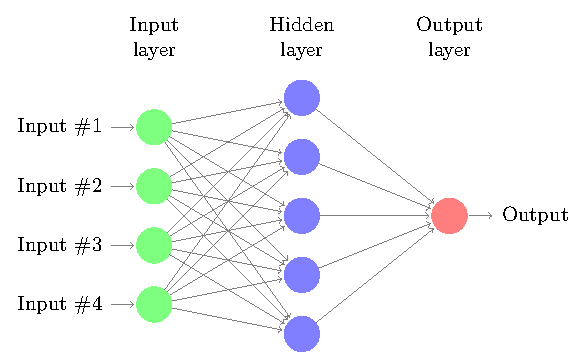
\includegraphics[width=.49\linewidth]{figures/neural-network.pdf}\label{fig:nnA}}  \hfill
% %% 	\subfloat[]{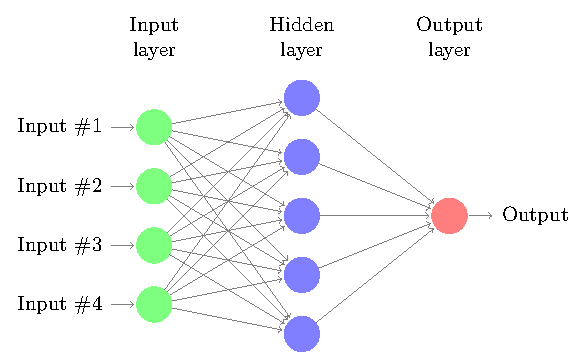
\includegraphics[width=.49\linewidth]{figures/neural-network.pdf}\label{fig:nnB}} \\
% %% \caption{\textbf{A.} A neural network. \textbf{B.} The same neural network.}
% %%   \label{fig:universes}
% %% \end{figure}

% %% \subsection{WP N: Writing the Dissertation}
% %% Writing the dissertation is planned. Things never go as planned.

% The proposed research mainly focuses on machine learning algorithms addressing the four main challenges in clinical data: heterogeneous sampling rate, irregular sampling rate, missing variables and different modalities of data.
% In the end these algorithms will be integrated into one framework which is the final goal of the proposal.
% The framework will be evaluated and compared with each algorithm alone to check if combining them will lead to improvement in performance.
% The following work packages present the outline of the main phases to tackle the research questions.

% \subsection{WP 1: Early-warning system for organ deterioration}
% In this workpackage we use ICU data collected from the ICUs of University Hospital Bern, which will be referred as Bern ICU data.
% The raw Bern ICU data come directly from the patient data management system (PDMS) of the hospital, which contains lots of artifacts caused by people misentering dates, values or variable IDs of the records.
% There are sometimes multiple records with different of the same variable for the same patients at the same time, which causes confusion because we do not know which one contains the correct measurement value.
% These artifacts need to be cleaned out before we use the data to train early-warning models.

% There exists more than 5000 variables in the Bern ICU data but not all are relevant to the organ deterioration tasks of interest, and also some are only used for short term like in clinical trails which lead to high sparseness.
% We only select variables that are most relevant to the prediction tasks as well as measured for most of the patients over most of the years in the dataset to reduce the sparseness in the final set of data that is used to train the early-warning system.
% The variable selection will be done by analyzing the statistics of the variables and with the professional knowledge from clinicians.

% After artifact cleaning and feature selection, we need to transform the data from tables to feature matrices that machine learning models can use as inputs.
% A patient will be represented by a matrix where each row corresponds to a time step and each column corresponds to a variable.
% In such matrices, there are many entries with missing values due to the heterogeneous and irregular sampling rate as well as the missing variables, which will be manually imputed.
% Labels of future organ deterioration will be computed from non-imputed data based on the definition provided by the clinicians. 
% Both non-sequential models, such as logistic regression or lightGBM, and sequential models like LSTMs will be used to predict organ deteriorations within the next 8 hours, the best one among which will be selected.
% This workpackage, where missing variables are imputed manually, establishes a baseline for the future work packages where deep learning models that can directly take non-imputed data as inputs. 

% This work is done in collaboration with Stephanie Hyland, Matthias H\"{u}ser, Martin Faltys and Tobias Merz.

% %% For the purpose of training and evaluation of the proposed algorithms and the final framework, clinical data are needed.
% %% One available clinical dataset is the ICU data collected from our collaborator, ``the University Hospital of Bern.
% %% Besides the Bern ICU dataset, two open-access ICU datasets will also be used: the MIMIC-III dataset \cite{saeed2011multiparameter} and the Philips eICU dataset \cite{mcshea2010eicu}.
% %% Since all the datasets used in the proposed research are collected from ICU, the data sampling rate usually ranges from every few minutes to once a few days.
% %% Table \ref{tbl:data} summarizes some basic information of these three datasets.
% %% \begin{table}[!ht]
% %%   \caption{Summary of the three ICU datasets we will use in the proposal.}
% %%   {\footnotesize
% %%   \begin{tabular}{p{0.225\textwidth} p{0.225\textwidth} p{0.225\textwidth} p{0.225\textwidth}}
% %%     \midrule
% %%     ~ & \textbf{MIMIC-III} & \textbf{Phillips eICU} & \textbf{University Hospital Bern} \\ \midrule
% %%     \textbf{No. of patients} & 46,520 & 139,367 & 55,476 \\ \midrule
% %%     \textbf{No. of variables} & 13,240 & 2,905 & 5,178 \\ \midrule
% %%     \textbf{No. of measurements} & $\approx 312\times10^6$ & $\approx 827\times10^6$ & $\approx 3,469\times10^6$ \\ \midrule
% %%     \textbf{Highest resolution} & $\approx 15$ minutes & $\approx 5$ minutes & $\approx 2$ minutes \\ \midrule
% %%     \textbf{Time range} & 2001 to 2012 & 2014 to 2015 & since 2005 \\ \midrule
% %%     \textbf{Demographics} & Patients at Beth Israel Deaconess Medical Centre (Boston, USA) & Patients from 459 critical care units across continental USA & Patients at University Hospital Bern (Switzerland) \\ \midrule
% %%   \end{tabular}}
% %%   \label{tbl:data}
% %% \end{table}

% %% While acquiring access to these ICU datasets is not difficult, the data do not come in a format that can be directly used by the proposed algorithms, so preprocessing the data into the desired format is an important task in this phase.
% %% Another problem is that the number of clinical variables is very large, however, a large amount of them were rarely observed.
% %% These rare variables may be observed only in some very specific patients or used in some short-term clinical trials, therefore not suitable for the general clinical problems.
% %% So one other important task in this phase is extracting commonly used and clinically important variables for general purposes.

% %% The raw ICU data directly from the patient data manangement system (PDMS) usually contain many artifacts caused by people misentering dates, values or variable ID of the observsations, or sometimes entering the same records multiple times and etc.
% %% While there are fewer artifacts in the MIMIC-III dataset and the eICU dataset because they might have been cleaned before people publish them, the Bern ICU dataset still contains quite some amount of artifacts that could significantly degrade the model peformance if ignored.
% %% Therefore, one additional task for the Bern ICU dataset is data cleaning.

% \paragraph{Deliverables}
% \begin{itemize}
% \item A set of programs that clean up the Bern ICU data, preprocess tables of ICU records and transform them into feature matrices.
% \item A medical journal paper on ICU Bern organ deterioration early-warning system.
% \end{itemize}

% \subsection{WP 2: Unsupervised representation learning from single data modality}
% This workpackage uses data from the Philips eICU dataset \cite{mcshea2010eicu}, which consists of 139367 patients and 2905 variables collected from 459 different critical care units across continental USA.
% Artifacts cleaning, feature selection, data format transformation and manual imputation also need to be applied, same as the preprocessing steps in WP 1.
% We compare non-sequential and sequential unsupervised learning techniques in terms of the representation performance in both reconstruction and prediction.
% In order to have a more objective evaluation on the generality of patients representations, we need to design a list of clinically related prediction tasks that covers a wide range of clinical concepts.
% The dynamic diagnosis and treatment records satisfy such requirement. 

% The non-sequential unsupervised representation learning techniques we use are PCA and vanilla autoencoder, and the sequential ones are variations of sequence-to-sequence model.
% Sequence-to-sequence models can be used as an autoencoder, i.e. the decoder reconstructs the input sequences; but it can also be used as a forecaster, which predict the future sequence of the current input sequences.
% Between a forecaster and an autoencoder with the same number of parameters, a forecaster has the advantage of ``seeing'' some future information than just the history during training, hence representations learned by the forecasters should be more predictive of the future events.
% Attention mechanism will also be added to the sequence-to-sequence forecaster under the intuition that feature values at each future time point may have higher relevance to only a local region of the input sequence. 

% \paragraph{Deliverables}
% \begin{itemize}
% \item A conference paper that benchmarks the unsupervised representation learning methods on medical time series.
% \end{itemize}

% \subsection{WP 3: Learning from multirate irregular time series}
% The data used for this workpackage are the commonly observed numerical variables.
% Missing variables will be imputed with global mean or expert-defined normal values.
% The data will be resampled to be on a fixed-interval time grid to remove the irregularity.
% Sampling rate of the data will be made sure to be in these three range: every few minutes, every few hours and once a day.
% In the baseline method, the time series will be imputed with forward-filling.

% The clinical problem of interest is learning representations that can be used to predict diagnosis/treatments in the future. 
% Different representation learning methods in a either supervised or unsupervised fashion will be studied in order to establish the best baseline.
% In the best representation learning model, the parts that takes the time series as inputs will be replaced with Phased LSTM, multi-rate LSTM and the proposed algorithm respectively, so that it will be able to take non-imputed multi-rate time series as inputs, and the former two will be the state-of-the-art baseline for the last one to compare against.
% The performance of the proposed method and the baselines will be evaluated on the representation performance in the diagnosis/treatment prediction tasks.

% Two naive baselines will be used in dealing with irregularity, in both of which standard LSTMs will be used, but one will ignore the irregularity by ``pretending'' that two consecutive observations always have a fixed time interval and the other uses data resampled to a fixed-interval time grid.
% Besides the two naive baselines, the proposed method will also be compared with T-LSTMs as the state-of-the-art baseline.
% \paragraph{Deliverables}
% \begin{itemize}
% \item Design, definition and implementation of the proposed algorithm.
% \item Two conference papers will be written presenting the proposed algorithms.
% \end{itemize}

% \subsection{WP 4: Learning from time series with missing variables}
% The data used in this work package will still be similar to those in WP 2, with the only difference that the missing variables will not be imputed.
% Since the research at this phase focuses on dealing with missing variables, the time-series will also be forward-imputed to remove the multirate aspect.
% The clinical problem is diagnosis prediction or medicine recommendation.

% Standard LSTMs will be applied to the data with missing variable values imputed by the statistical global mean or the expert-defined normal values.
% Methods and metrics to measure the similarity between time series will be designed so the temporal components can also be incorporated into the CF framework for the clinical problem.
% \paragraph{Deliverables}
% \begin{itemize}
% \item Design of the similarity measurement method and metric for time series.
% \item A conference paper will be written presenting CF over clinical time series with missing variables.
% \end{itemize}

% \subsection{WP 5: Representation learning from heterogeneous data modalities}
% In this work package, we will implement a joint model that combines Med2Vec \cite{choi2016multi} and the representation learning algorithm for numerical clinical variables developed in WP 2.
% Representations learned from the joint model will be compared with the Med2Vec representations and WP-2 representations in terms of their prediction performance in the organ deterioration early-warning task mentioned in WP 1. 

% %% In this work package, the methods from WP 2, 3, 4 will be integrated into a united model that uses only numerical time-series data as input.
% %% Time series of texts will be encoded into time series of word embeddings using GloVe, and time series of medical codes will be encoded by Med2Vec.
% %% The time series of embeddings will be treated the same as the numerical time series and be input to the aforementioned combined time-series model.
% %% The entire framework will be compared with the combined model that only uses numerical clinical variables to check if incorporating more data will improve the performance.
% \paragraph{Deliverables}
% \begin{itemize}
% \item A represenation model that take both numerical clinical variables and medical codes as inputs.
% \end{itemize}

% \subsection{WP 6: Writing the Dissertation}
% Writing dissertation to summarize all the previous works.
\label{sec:detailed_work_plan}

\onlyIfMaxPages{\pagebreak}
\section{Progress to Date\onlyIfMaxPages{ (min. 1/4 page)}}


\subsection{WP 1: sequence similarity sketching}
The publication outlining the method developed for work package 1 will be published in the proceedings of RECOMB 2021~\cite{joudaki2020fast}. Furthermore, the reference code implementation of this method, along with the code for the experiments, is now publicly avaible~\footnote{The source code is available at https://github.com/ratschlab/Project2020-seq-tensor-sketching}. 

When experimented against synthetically generated sequences, \emph{Tensor Sketching} technique demonstrates a higher accuracy than the other assessed sketching methods, particularly when the mutation rate is high. Furthermore, sketches can be computed in a dynamic fashion, allowing us to compute sketches of all substrings of a sequences in linear time. This dynamic sketches are then leveraged to design a better sketch, termed \emph{Tensor Slide Sketch}, that shows the highest accuracy among the methods assessed. Finally, tensor sketching can be viewed as a framework to tackle a wide range of relevant bioinformatics problems, since it is straightforward to extend tensor sketching to different settings.

My contributions were developing the original idea of tensor sketching, tensor slide sketching, and design of the experimental setup that was eventually used in the publication, and eventually writing the publication along with the co-authors.  Furthermore, I implemented the first version of the tensor sketching in C++, which served the basis of the current reference code.

% \subsection{WP 2: Phylogeny reconstruction}
% The sketching framework is currently integrated into a phylogeny reconstruction, with the aim of improving the performance of MASH over a dataset of virus genomes. 

% \onlyIfMaxPages{\pagebreak}
% \section{Schedule\onlyIfMaxPages{ (min. 1/4 page)}}
% %% A schedule showing clearly when you started the PhD, the work packages completed or under way and the envisaged start and end times of the future work packages should be included. This should include estimates of when the thesis will be completed, including the writing of the thesis report.
The research schedule for four years is presented in Figure \ref{fig:timeSchedule}.
It comprises the six work packages previously discussed.
\begin{figure}[h]
  \centering
  \def\svgwidth{.7\columnwidth}
	{\small\import{figures/}{timeSchedule_pdf.tex}}
	\caption{Research Plan for 4 years.} 
  \label{fig:timeSchedule}
\end{figure}






\pagebreak
\section{References\onlyIfMaxPages{ (max. 1 page)}}
%% A list of papers referenced in the description of the state-of-the-art should be included. Since the research plan is intended to be a summary document, it is not necessary to include large lists of all papers that you have read, but rather to reference key papers in your area of research. 
\printbibliography[heading=none]

% \pagebreak
% \section{Additional Information}
% %% The ETH regulations taking effect from November 2013 state that the following additional information must be included in research plans:
%% \begin{itemize}
%%  \item Expected publications
%%  \item Teaching duties
%%  \item Other duties
%% \end{itemize}
%% This section is indented to list any special conditions stipulated by your supervisor such as a publication in a specific conference or journal, or special teaching and administration duties. If there are none, you can simply write ``no special requirements''.

\paragraph{Accepted works}
\begin{itemize}
\item Predicting Circulatory System Deterioration in Intensive Care Unit Patients, \textit{Joint Workshop on Artificial Intelligence in Health 2018}. (Workshop paper, \textbf{WP 1})
\item A Machine Learning-based Early Warning System for Circulatory System Deterioration in Intensive Care Unit Patients, \textit{AMIA 2018 Annual Symposium}. (Podium abstract, \textbf{WP 1})
\end{itemize}
\paragraph{Expected publications}
\begin{itemize}
\item A medical journal paper on ICU Bern organ deterioration early warning system project. (\textbf{WP 1})
\item A conference paper that benchmarks the unsupervised representation learning methods on medical time series, \textit{submitted to NIPS 2018}. (\textbf{WP 2})
\item A conference paper on representation learning with the proposed algorithm that will address the multirate challenges in medical time series. (\textbf{WP 3})
\item A conference paper describing the proposed method to deal with the irregularity issues in medical time series. (\textbf{WP 3})
\item A conference paper presenting the proposed method to handle the missing variable problems in medical time series. (\textbf{WP 4})
\end{itemize}
\paragraph{Teaching duties}
The teaching plan is to TA one course from the machine learning institute of ETH every semester.
\paragraph{Student project supervision}
The student project supervision plan is to supervise one master project maybe along with a short-term student project each year.
So far, I have supervised one master project on spliceogenicity prediction from Aug. 2017 to Feb. 2018, and am currently supervising another one on cancer mutational signatures which started in Jun. 2018.
\paragraph{Other projects}
\begin{itemize}
\item \textbf{Testing for differential protein abundance from DIA data}. The goal of this project is to develop new methods for identifying differentially expressed proteins from the mass spectrometry (MS) data.
A paper on this project will be expected in winter 2018.
\end{itemize}


\pagebreak
\section{Study Plan}
%% Students may include a proposed study plan for the required 12 credits (see the department guidelines for details of how these credits can be earned). Including a proposed study plan at this stage allows it to be approved in advance.
The study plan for getting 12 credits is shown in Table~\ref{tbl:study_plan}.
\begin{table}[!ht]
  \centering
  \begin{tabular}{l c c}
    \midrule
    % \textbf{Course} & \textbf{Credit} & \textbf{Status}\\ \hline\midrule
        \textbf{Course title} & \textbf{CP} & \textbf{Status}\\\midrule
    Advanced Algorithms & 9 & not yet \\\midrule
    Graph Theory & 5 &  enrolled \\\midrule
    % Advanced Graph Algorithms & 8 & not yet\\\hline\midrule
    \textbf{Sum} & 14\\
    \midrule
  \end{tabular}
\caption{Study plan, CP: credit points.}
  \label{tbl:study_plan}

\end{table}


\section*{}

\rule{\textwidth}{1pt}\vspace{3em}
\noindent\begin{tabular}{ll}
\makebox[2.5in]{\hrulefill} & \makebox[2.5in]{\hrulefill}\\    Ph.D. Candidate & Place, Date\\[8ex]% adds space between the two sets of signatures
\makebox[2.5in]{\hrulefill} & \makebox[2.5in]{\hrulefill}\\    Supervisor & Place, Date\    \end{tabular}



%% Dokument ENDE %%%%%%%%%%%%%%%%%%%%%%%%%%%%%%%%%%%%%%%%%%%%%%%%%%%%%%%%%%
\end{document}

\
